
\subsubsection{Multi-Layer Perceptron}

Next, the \texttt{neuralnet} package \cite{neuralnet} is used to fit a multi-layer perceptron network to the earthquake data.  After pre-processing to split the data 70/30 for training and testing respectively, the network architecture is defined as a three-layer network with 5 neurons in each hidden layer.  The function uses resilient backpropagation by default and sigmoid activation between layers.
%------------------comment--------------------------------------------
\begin{comment}
\begin{Shaded}
\begin{Highlighting}[]
\FunctionTok{set.seed}\NormalTok{(}\DecValTok{4723}\NormalTok{)}

\CommentTok{\#shuffle the data}
\NormalTok{df }\OtherTok{\textless{}{-}}\NormalTok{ earthquakes\_log[}\FunctionTok{sample}\NormalTok{(}\FunctionTok{nrow}\NormalTok{(earthquakes\_log)), ]}

\CommentTok{\#Extract 70\% of data into train set and the remaining 30\% in test set}
\NormalTok{train\_test\_split }\OtherTok{\textless{}{-}} \FloatTok{0.7} \SpecialCharTok{*} \FunctionTok{nrow}\NormalTok{(df)}
\NormalTok{train }\OtherTok{\textless{}{-}}\NormalTok{ df[}\DecValTok{1}\SpecialCharTok{:}\NormalTok{train\_test\_split,]}
\NormalTok{test }\OtherTok{\textless{}{-}}\NormalTok{ df[(train\_test\_split}\SpecialCharTok{+}\DecValTok{1}\NormalTok{)}\SpecialCharTok{:} \FunctionTok{nrow}\NormalTok{(df),]}

\NormalTok{mlp }\OtherTok{\textless{}{-}} \FunctionTok{neuralnet}\NormalTok{(freqc }\SpecialCharTok{\textasciitilde{}}\NormalTok{ mag,}
                 \AttributeTok{stepmax =} \FloatTok{1e+06}\NormalTok{,}
                 \AttributeTok{data =}\NormalTok{ train,}
                 \AttributeTok{hidden =} \FunctionTok{c}\NormalTok{(}\DecValTok{5}\NormalTok{,}\DecValTok{5}\NormalTok{))}

\CommentTok{\#prediction for magnitude 9.1}
\NormalTok{p }\OtherTok{\textless{}{-}} \FunctionTok{predict}\NormalTok{(mlp, }\AttributeTok{newdata =} \FunctionTok{data.frame}\NormalTok{(}\AttributeTok{mag =} \FloatTok{9.1}\NormalTok{))}
\DecValTok{1}\SpecialCharTok{/}\DecValTok{10}\SpecialCharTok{\^{}}\NormalTok{p}
\end{Highlighting}
\end{Shaded}

\begin{verbatim}
##          [,1]
## [1,] 3212.887
\end{verbatim}
\end{comment}
%---------------------------------------------------------------------
Using this neural network model, the expected frequency of a magnitude
9.1 earthquake would be one every 3,212.89 years (See Appendix).  That's less frequent than the base linear model from before, and more frequent than the second order polynomial model that accounted for the curvature of the data.  Still it may not be enough to convince the Fukushima engineering officials to build a stronger reactor.  A plot of the data is shown below:

\begin{figure}[H]
    \center
    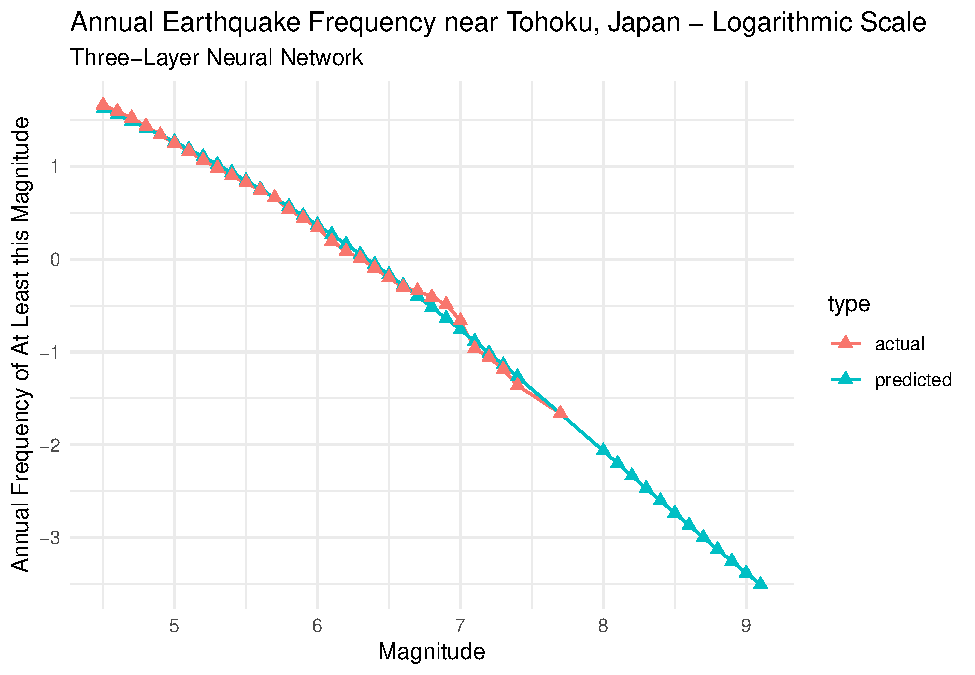
\includegraphics[width=0.8\linewidth]{earthquakes_files/figure-latex/unnamed-chunk-8-1.pdf}
   % \vspace{-10pt}
    \caption{\footnotesize{Actual data points plotted with MLP-predicted values for all data points, with appended predicted magnitudes for sequential series of magnitude 8.0 - 9.1 by 0.1}}
    \label{tohoku_mlp}
\end{figure}


\subsubsection{Capacity Simulation for Neural Network}

Adding more neurons or more layers to a neural network can increases model capacity. Recall that a higher capacity model is able to fit more functions, but requires a lot more data to be able to generalize.  This is measured by the \textit{generalization gap}, which is a measure of the difference between the training error and test error. Ideally, a good model has a low training error, low test error, and a small generalization gap.

To determine the best model from a set of possible networks, three networks were fit to the same data with 70/30 train/test split.  Each model had the same architecture and the same number of neurons (5) in each layer.  The only difference between each network was the number of hidden layers. Table \ref{gengapt} displays the error measurements for a network with one, two, and three hidden layers. Moving from the first network to the second, training and test error are smaller and the generalization gap is minimized.  That this value increases moving from the second to the third network is indicative that the three-layer model is overfit to the data.


% latex table generated in R 4.2.2 by xtable 1.8-4 package
% Thu Apr 27 13:43:54 2023
\begin{table}[ht]
\centering
\begin{tabular}{rrrr}
  \hline
 & 1 Hidden Layer & 2 Hidden Layers & 3 Hidden Layers \\ 
  \hline
Test Error & 0.0098383338 & 0.0086557953 & 0.0111406131 \\ 
Train Error & 0.0380235026 & 0.0178080209 & 0.0290913220 \\ 
Generalization Gap & 0.0281851688 & 0.0091522255 & 0.0179507089 \\ 
   \hline
\end{tabular}
\caption{\footnotesize Error measurements of neural networks with identical structure less the number of hidden layers.  Among these three, the network with two hidden layers is capacity because it has the smallest difference between training and test error.}
\label{gengapt}
\end{table}

Based on this table, the model used in the example above is the optimal fit.  Perhaps with further adjustments to the network architecture (i.e. layer sizes or activations used) an even better model could be fit based on relative error measurements; but to find the best neural network model for a specialized case is beyond the scope of this thesis.  One thing to note however is that this model is devoid of any regularization technique.  In a later section, the same example will be revisited using \textit{weight decay} in which parameters $\alpha$ and $\beta$ are determined from a Bayesian approach.  In the meantime, this thesis will summarize some important and methods of Bayesian Statistics.

%------------------comment--------------------------------------------
\begin{comment}
The code below builds different networks to answer the same question in predicting Tohoku earthquake frequencies.  For each model, the test error is calculated by sums of squares.  Three networks are made, each with one more layer than the previous and each with 5 neurons per hidden layer.

\begin{Shaded}
\begin{Highlighting}[]
\FunctionTok{set.seed}\NormalTok{(}\DecValTok{4723}\NormalTok{)}
\CommentTok{\#{-}{-}{-}one hidden layer{-}{-}{-}}
\NormalTok{mlp }\OtherTok{\textless{}{-}} \FunctionTok{neuralnet}\NormalTok{(freqc }\SpecialCharTok{\textasciitilde{}}\NormalTok{ mag,}
                 \AttributeTok{stepmax =} \FloatTok{1e+06}\NormalTok{,}
                 \AttributeTok{data =}\NormalTok{ train,}
                 \AttributeTok{hidden =} \FunctionTok{c}\NormalTok{(}\DecValTok{5}\NormalTok{))}

\CommentTok{\#predictions on test data}
\NormalTok{pps }\OtherTok{\textless{}{-}} \FunctionTok{predict}\NormalTok{(mlp, }\AttributeTok{newdata =} \FunctionTok{data.frame}\NormalTok{(}\AttributeTok{mag =}\NormalTok{ test}\SpecialCharTok{$}\NormalTok{mag))}

\CommentTok{\#SSE to get test error}
\NormalTok{TestErr1 }\OtherTok{\textless{}{-}} \FunctionTok{sum}\NormalTok{((pps }\SpecialCharTok{{-}}\NormalTok{ test}\SpecialCharTok{$}\NormalTok{freqc)}\SpecialCharTok{\^{}}\DecValTok{2}\NormalTok{)}
\NormalTok{TrainErr1 }\OtherTok{\textless{}{-}}\NormalTok{ mlp}\SpecialCharTok{$}\NormalTok{result.matrix[}\DecValTok{1}\NormalTok{,]}

\FunctionTok{set.seed}\NormalTok{(}\DecValTok{4723}\NormalTok{)}
\CommentTok{\#{-}{-}{-}two hidden layers{-}{-}{-}}
\NormalTok{mlp }\OtherTok{\textless{}{-}} \FunctionTok{neuralnet}\NormalTok{(freqc }\SpecialCharTok{\textasciitilde{}}\NormalTok{ mag,}
                 \AttributeTok{stepmax =} \FloatTok{1e+06}\NormalTok{,}
                 \AttributeTok{data =}\NormalTok{ train,}
                 \AttributeTok{hidden =} \FunctionTok{c}\NormalTok{(}\DecValTok{5}\NormalTok{,}\DecValTok{5}\NormalTok{))}

\CommentTok{\#predictions on test data}
\NormalTok{pps }\OtherTok{\textless{}{-}} \FunctionTok{predict}\NormalTok{(mlp, }\AttributeTok{newdata =} \FunctionTok{data.frame}\NormalTok{(}\AttributeTok{mag =}\NormalTok{ test}\SpecialCharTok{$}\NormalTok{mag))}

\CommentTok{\#SSE to get test error}
\NormalTok{TestErr2 }\OtherTok{\textless{}{-}} \FunctionTok{sum}\NormalTok{((pps }\SpecialCharTok{{-}}\NormalTok{ test}\SpecialCharTok{$}\NormalTok{freqc)}\SpecialCharTok{\^{}}\DecValTok{2}\NormalTok{)}
\NormalTok{TrainErr2 }\OtherTok{\textless{}{-}}\NormalTok{ mlp}\SpecialCharTok{$}\NormalTok{result.matrix[}\DecValTok{1}\NormalTok{,]}

\FunctionTok{set.seed}\NormalTok{(}\DecValTok{4723}\NormalTok{)}
\CommentTok{\#{-}{-}{-}three hidden layers{-}{-}{-}}
\NormalTok{mlp }\OtherTok{\textless{}{-}} \FunctionTok{neuralnet}\NormalTok{(freqc }\SpecialCharTok{\textasciitilde{}}\NormalTok{ mag,}
                 \AttributeTok{stepmax =} \FloatTok{1e+06}\NormalTok{,}
                 \AttributeTok{data =}\NormalTok{ train,}
                 \AttributeTok{hidden =} \FunctionTok{c}\NormalTok{(}\DecValTok{5}\NormalTok{,}\DecValTok{5}\NormalTok{,}\DecValTok{5}\NormalTok{))}

\CommentTok{\#predictions on test data}
\NormalTok{pps }\OtherTok{\textless{}{-}} \FunctionTok{predict}\NormalTok{(mlp, }\AttributeTok{newdata =} \FunctionTok{data.frame}\NormalTok{(}\AttributeTok{mag =}\NormalTok{ test}\SpecialCharTok{$}\NormalTok{mag))}

\CommentTok{\#MSE to get test error}
\NormalTok{TestErr3 }\OtherTok{\textless{}{-}} \FunctionTok{sum}\NormalTok{((pps }\SpecialCharTok{{-}}\NormalTok{ test}\SpecialCharTok{$}\NormalTok{freqc)}\SpecialCharTok{\^{}}\DecValTok{2}\NormalTok{)}
\NormalTok{TrainErr3 }\OtherTok{\textless{}{-}}\NormalTok{ mlp}\SpecialCharTok{$}\NormalTok{result.matrix[}\DecValTok{1}\NormalTok{,]}

\CommentTok{\#View results}
\NormalTok{TestError }\OtherTok{\textless{}{-}} \FunctionTok{cbind}\NormalTok{(TestErr1,TestErr2,TestErr3)[}\DecValTok{1}\SpecialCharTok{:}\DecValTok{3}\NormalTok{]}
\NormalTok{TrainError }\OtherTok{\textless{}{-}} \FunctionTok{cbind}\NormalTok{(TrainErr1, TrainErr2, TrainErr3)[}\DecValTok{1}\SpecialCharTok{:}\DecValTok{3}\NormalTok{]}
\NormalTok{GeneralizationGap }\OtherTok{\textless{}{-}}\NormalTok{ TrainError }\SpecialCharTok{{-}}\NormalTok{ TestError}

\FunctionTok{data.frame}\NormalTok{(}\FunctionTok{rbind}\NormalTok{(TestError,TrainError,GeneralizationGap))}
\end{Highlighting}
\end{Shaded}

\begin{verbatim}
##                            X1          X2         X3
## TestError         0.009838334 0.008655795 0.01114061
## TrainError        0.038023503 0.017808021 0.02909132
## GeneralizationGap 0.028185169 0.009152226 0.01795071
\end{verbatim}
\end{comment}
%---------------------------------------------------------------------
